\documentclass[a4paper]{report}

\usepackage[utf8]{inputenc}
\usepackage[T1]{fontenc}
\usepackage[francais]{babel}
\usepackage{graphicx}
\usepackage{caption}
\usepackage{float}
\usepackage{pdfpages} 
\usepackage{listings}
\usepackage{color}
\usepackage{array}
\usepackage{geometry}
\usepackage{dsfont}
\usepackage{amsmath}
\usepackage{amsfonts, amssymb}
\usepackage{fancyhdr}
\usepackage{lastpage}
\usepackage{todonotes}
\usepackage{url}
\usepackage{subfigure}
\usepackage{verbatim}
\usepackage{ifthen}
\usepackage{xstring}
\usepackage{siunitx}

\usepackage[pdftex,           %%% hyper-references for pdflatex
bookmarks=true,               %%% generate bookmarks ...
bookmarksnumbered=true,       %%% ... with numbers
hypertexnames=false,          %%% needed for correct links to figures
breaklinks=true,              %%% break links if exceeding a single line
colorlinks=true,              %%% links are colored
citecolor=blue,               %%% color of cite links
linkcolor=black,               %%% color of hyperref links
menucolor=black,              %%% color of Acrobat Reader menu buttons
urlcolor=magenta,             %%% color of page of \url{...}
pdfstartview=FitH]{hyperref}

% commande pour référencer plus explicitement:
\newcommand*{\fullref}[1]{\hyperref[{#1}]{\autoref*{#1} \nameref*{#1}}}
\newcommand*{\titleref}[1]{\hyperref[{#1}]{\ref*{#1} \nameref*{#1}}}

%\usepackage{nameref}
\usepackage{amsfonts,amssymb}
\usepackage{amsmath}
%\usepackage{verbatim} déjà déclaré plus haut
\usepackage{xspace}
%\usepackage{glossaries}
%\addto\captionsfrench{%
%    \renewcommand*{\glossaryname}{Glossaire}}


\lstset{
language=C,
basicstyle=\footnotesize,
numbers=left,
numberstyle=\normalsize,
numbersep=15pt,
}
\pagestyle{fancy}
\lhead{\leftmark}
\rhead{\rightmark}
\lfoot{François Der Hovsepian}
\cfoot{\thepage/\pageref{LastPage}}
\rfoot{Rapport sur l'état du framework AngioTK}

% bibliographie
\usepackage[backend=biber,style=alphabetic]{biblatex}
\providecommand*{\footcite}{\fc}
\bibliography{bib/bibliography.bib}

% symboles mathématiques
\newcommand{\N}{{\mathbb{N}}}
\newcommand{\Z}{{\mathbb{Z}}}
\newcommand{\R}{{\mathbb{R}}}
\newcommand{\vecteur}{\overrightarrow}
\newcommand{\vect}[1]{\boldsymbol{#1}}


% abréviations
\newcommand{\cad}{c'est-à-dire\xspace}
\newcommand{\ioT}{Formats supportés\xspace}
\newcommand{\argsT}{Paramètres\xspace}
\newcommand{\etatg}{État général\xspace}

% 
\newcommand \sw[1] {\texttt{#1}\xspace}
\newcommand \sourcepath[1 ]{\path{#1}\xspace}
\newcommand \rorpo {\sw{RORPO}\xspace}
\newcommand \vmtk {\sw{VMTK}\xspace}
\newcommand \gmsh {\sw{Gmsh}\xspace}
\newcommand \paraview {\sw{Paraview}\xspace}
\newcommand \cts {\sw{component\_tree\_segmentation}\xspace}
\newcommand \runpy {\sw{runAngioTKPipeline.py}\xspace}
\newcommand \masterpy {\sw{master.py}\xspace}
\newcommand \summaryHtml {\sw{summary.html}\xspace}


% marqueurs
\newcommand \tbv {\textcolor{red}{(?)}\xspace}
\newcommand \execname[1] {\texttt{#1}\xspace}
\newcommand \argfont {\texttt}
\newcommand \argtypefont[1] {\textcolor{olive}{#1}}
\newcommand \argvaluefont[1] {\textcolor{gray}{#1}}
\newcommand \argdescriptionfont[1] {\textcolor{teal}{#1}}
\newcommand {\cfgfont} {\texttt}
\newcommand \cfgtypefont[1] {\textcolor{olive}{#1}}
\newcommand \cfgvaluefont[1] {\textcolor{gray}{#1}}
\newcommand \cfgdescriptionfont[1] {\textcolor{teal}{#1}}
\newcommand \cfgsectiondescriptionfont[1] {\textcolor{violet}{#1}}
\newcommand \cfgcommentfont[1] {\textcolor{violet}{#1}}

% formats de fichier
\newcommand {\mha} {MetaImage (.mha)\xspace}
\newcommand {\nii} {NIfTI (.nii)\xspace}
\newcommand {\stl} {STereoLithography (.stl)\xspace}
\newcommand {\msh} {MSH (.msh)\xspace}
\newcommand {\desc} {desc (.desc)\xspace}
\newcommand {\pointpair} {texte contenant des paires de points (.pointpair.data)\xspace}
\newcommand {\vtk} {VTK (.vtk)\xspace}
\newcommand {\html} {html\xspace}
\newcommand {\json} {json\xspace}

% répertoires
\newcommand {\resultsDataBase} {\textit{resultsDataBase}}

\makeatletter
% ----------------------------------- commande \iolist ------------------------------------
% Détail des paramètres d'un programme en ligne de commande: fonction pour l'utilisateur (contient un nombre impair d'arguments: des couples {argument}{description} et un argument  final pour clore la liste: \stoparg
\newcommand \iolist[2] {% (On commente cette ligne pour pouvoir la sauter.)
\begin{itemize}
\item \texttt{Entrée}: {#1}
\item \texttt{Sortie}: {#2}
\end{itemize}
}
\makeatother

\makeatletter
% ----------------------------------- commande \args ------------------------------------
% Détail des paramètres d'un programme en ligne de commande: fonction pour l'utilisateur (contient un nombre impair d'arguments: des couples {argument}{description} et un argument  final pour clore la liste: \stoparg
\newcommand{\args}{% (On commente cette ligne pour pouvoir la sauter.)
\begin{itemize}
\@argstest
}
\newcommand \@argstest{%
\@ifnextchar\stoparg{\@argsend}{\@argscouple}
}
\newcommand \@argscouple[4]{%
\StrLen{#1}[\argLength]% on stocke la longueur d'abord /!\ important, \StrLen ne peut pas être incluse (nested) dans le 'if'
\ifthenelse{\equal{\argLength}{1}}% On distingue 2 cas:
{\@argscoupleshort{#1}{#2}{#3}{#4}}% argument court (une seule lettre, comme -i) 
{\@argscouplelong{#1}{#2}{#3}{#4}}% et argument long (--input)
\@argstest
}
\newcommand \@argscoupleshort[4]{%
\item[] \argfont{-#1}: \argvaluefont{#2} (\argtypefont{#3}) \argdescriptionfont{#4}
}
\newcommand \@argscouplelong[4]{%
\IfSubStr{#1}{<}% On distingue entre <input> et --input
{\item[] \argfont{#1>}: \argvaluefont{#2} (\argtypefont{#3}) \argdescriptionfont{#4}}% 
{\item[] \argfont{-{}-#1}: \argvaluefont{#2} (\argtypefont{#3}) \argdescriptionfont{#4}}
}
\newcommand \@argsend[1]{%
\end{itemize}
}
\makeatother

\makeatletter
% --------------------------------- commande \configfile ------------------------------------
% Détail des paramètres d'un fichier de configuration: fonction pour l'utilisateur (contient un nombre impair d'arguments: des couples {argument}{description} et un argument  final pour clore la liste: \stopfile
\newcommand{\configfile}{% (On commente cette ligne pour pouvoir la sauter.)
\begin{itemize}
\@configfiletest
}
\newcommand\@configfiletest{%
\@ifnextchar\stopfile{\@configfileend}{\@configfilearg}
}
\newcommand\@configfilearg[4]{%
\IfSubStr{#1}{[}{ \item[] \cfgfont{#1} \# \cfgsectiondescriptionfont{#2}\xspace}% section
{\IfSubStr{#1}{//}{ \item[] \cfgcommentfont{#1} \xspace}% commentaire
{ \item[] \cfgfont{#1}=\cfgvaluefont{#2} \# (\cfgtypefont{#3})  \cfgdescriptionfont{#4}\xspace}}% parametre
\@configfiletest
}
\newcommand\@configfileend[1]{%
\end{itemize}
}
\makeatother


% raccourcis chemins
\newcommand{\chpath}{}
\newcommand{\secpath}{}
\newcommand{\imgpath}{}

\title{Rapport sur l'état du framework AngioTK.}
\author{François Der Hovsepian}
\date{\today}

\makeindex
%\makeglossaries

%--------------------------------------------------begin document----------------------------------------

\begin{document}


\makeatletter

\begin{titlepage}

\centering
\Large
%Rapport de stage\\
%Master 2 de Calcul Scientifique et Mathématiques de l'Information

\vfill

%\includegraphics[scale=0.3]{logo-uds.png}
\vfill
\hrule
\vfill

\Huge\@title\\
\vfill

\huge
\hrule
\vfill
\small\@author\\
%\vspace{15pt}
%\vfill
%\Large
%\@date
\vfill

\end{titlepage}
 
\makeatother




%\include{0-abstract/abstract}
%\include{0-abstract/merci}

\tableofcontents

\chapter{Introduction}
\label{chap:intro}

\section{Contexte scientifique et problématique}

AngioTK s'inscrit dans le cadre du projet VIVABRAIN...

\subsection{Objectifs}

Le but est, en partant d'IRM de patients, de reconstruire des modèles 3D du système vasculaire cérébral, puis de pouvoir y effectuer des simulations d'écoulements sanguins et des simulations d'IRM (angiographies virtuelles).


\renewcommand{\chpath}{2-architecture/}
\renewcommand{\imgpath}{\chpath img/}
\renewcommand{\secpath}{\chpath}
\chapter{Architecture}
\label{chap:archi}

\newcommand{\imgW}{.8}

Dans cette partie, nous présentons l'architecture du projet, et détaillons en particulier la reconstruction de modèles. AngioTK prend la forme d'une chaîne de traitement (on parle de pipeline logiciel) qui prend une image IRM de cerveau en entrée et lui fait traverser une succession d'étapes menant à la simulation d'IRM. Chacune de ces étapes correspond à un logiciel à part entière (ou brique logicielle) inséré dans la chaîne.

\section{Images IRM à traiter}

Afin de pouvoir mettre au point et tester le pipeline, plusieurs images IRM ont été utilisées. Elles sont regroupées dans 3 bases de données.

\subsection{Base 1}

La base 1 contient 71 IRM...

\subsection{Base 2}

La base 2 contient 38 IRM acquises dans le cadre du projet. La taille des voxels est $0,8\times0,8\times0,8$ \SI{}{\milli\meter\cubed}

\subsection{Base 3}

La base 3 rassemble les IRM de 94 patients. Ces données proviennent de la base de donnée publiée par Elizabeth Bullitt (\href{http://www.insight-journal.org/midas/community/view/21}{http://www.insight-journal.org/midas/community/view/21}). Les angiographies ont été acquises avec des voxels de $0,5\times0,5\times0,8$ \SI{}{\milli\meter\cubed}.

%\newpage

\section{Pipeline de reconstruction de modèle}

\subsection{Principe général}

La reconstruction de modèle 3D et la génération de maillage ont lieu en plusieurs étapes. L'organisation de ces étapes suit le schéma général suivant:

\ 

On part d'une image 3D (IRM), on isole les structures d'intérêt (les vaisseaux sanguins) dans cette image 3D et on extrait leur surface. Enfin, on en génère un maillage du volume correspondant.

\ 

Cependant, des étapes intermédiaires sont nécessaires afin d'obtenir un résultat acceptable en vue des simulations. Dans la suite, le détail de l'architecture du pipeline permet de comprendre pourquoi.

\ 

\subsection{Filtrage des images}

L'isolation des structures d'intérêt est assurée par le logiciel \rorpo. Il filtre les images 3D pour mettre en valeur les structures tubulaires qu'elles contiennent.

\begin{figure}[H]
\begin{center}
  \subfigure[]{ \includegraphics[width=.8\linewidth]{\imgpath 0_mri}\label{fig:0mri}}
  \subfigure[]{ \includegraphics[width=.8\linewidth]{\imgpath 1_rorpo}\label{fig:1rorpo}}
\caption{Image IRM avant \subref{fig:0mri} et après filtrage \subref{fig:1rorpo}.
}
\end{center}
\label{fig:rorpo}
\end{figure}

\subsection{Extraction de surface}

À partir de l'image filtrée, on peut extraire la surface des vaisseaux sanguins. Cependant, on obtient une surface très irrégulière (c'est une conséquence du bruit présent à l'origine dans l'image). C'est pourquoi on ne passe pas directement à la génération de maillage.

\begin{figure}[H]
\begin{center}
  \subfigure{ \includegraphics[width=\imgW \linewidth]{\imgpath 2_sfi}\label{fig:2sfi}}
\caption{Surface extraite.% \subref{fig:2sfi}.
}
\end{center}
\label{fig:sfi}
\end{figure}

\subsection{Définition des lignes centrales}

L'idée actuellement implantée consiste à se servir de ce modèle imparfait pour trouver et extraire les lignes centrales des vaisseaux sanguins. L'idée est ensuite de s'en servir pour reconstruire un modèle plus régulier et débarrassé du bruit.

\begin{figure}[H]
\begin{center}
  \subfigure{ \includegraphics[width=\imgW \linewidth]{\imgpath 3_cl}}%\label{fig:3cl}}
\caption{Lignes centrales d'une partie du modèle.% \subref{fig:3cl}.
}
\end{center}
\label{fig:cl}
\end{figure}

\subsection{Génération d'une nouvelle image 3D}

Ces lignes centrales servent d'abord à créer une image 3D (semblable à l'IRM de départ). Cette image de synthèse ne contiendra que des vaisseaux sanguins reconstruits à partir des lignes centrales. Les avantages sont l'absence de bruit et la régularité obtenue.

\begin{figure}[H]
\begin{center}
  \subfigure{ \includegraphics[width=\imgW \linewidth]{\imgpath 4_ifcl}}%\label{fig:4ifcl}}
\caption{Image générée à partir des lignes centrales.% \subref{fig:4ifcl}.
}
\end{center}
\label{fig:ifcl}
\end{figure}

\subsection{Deuxième extraction de surface}
\label{arch:sfi2}

Une deuxième extraction de surface, en utilisant l'image 3D générée, permet alors d'obtenir un modèle 3D très régulier.

\begin{figure}[H]
\begin{center}
  \subfigure{ \includegraphics[width=\imgW \linewidth]{\imgpath 5_sfi2}}%\label{fig:5sfi2}}
\caption{Surface extraite.% \subref{fig:5sfi2}.
}
\end{center}
\label{fig:sfi2}
\end{figure}

\subsection{Traitement de surface}

On remaille la surface et on ouvre les extrémités des vaisseaux sanguins.

\begin{figure}[H]
\begin{center}
  \subfigure{ \includegraphics[width=\imgW \linewidth]{\imgpath 6_sm}}%\label{fig:6sm}}
\caption{Maillage surfacique avec extrémités ouvertes.% \subref{fig:6sm}.
}
\end{center}
\label{fig:vm}
\end{figure}

\subsection{Génération de maillage volumique}
\label{arch:vm}

On remaille le volume et on génère un fichier de description pour les simulations. On peut également extruder une couche d'épaisseur pour la paroi des vaisseaux sanguins.

\begin{figure}[H]
\begin{center}
  \subfigure{ \includegraphics[width=\imgW \linewidth]{\imgpath 7_vm}}%\label{fig:7vm}}
\caption{Maillage volumique.% \subref{fig:7vm}.
}
\end{center}
\label{fig:vm}
\end{figure}

\newcommand{\figpart}{.5}
\newcommand{\hpart}{1.}

\begin{center}
 \begin{figure}[H]
	\begin{minipage}[t]{\figpart \linewidth}
            	\centering
            	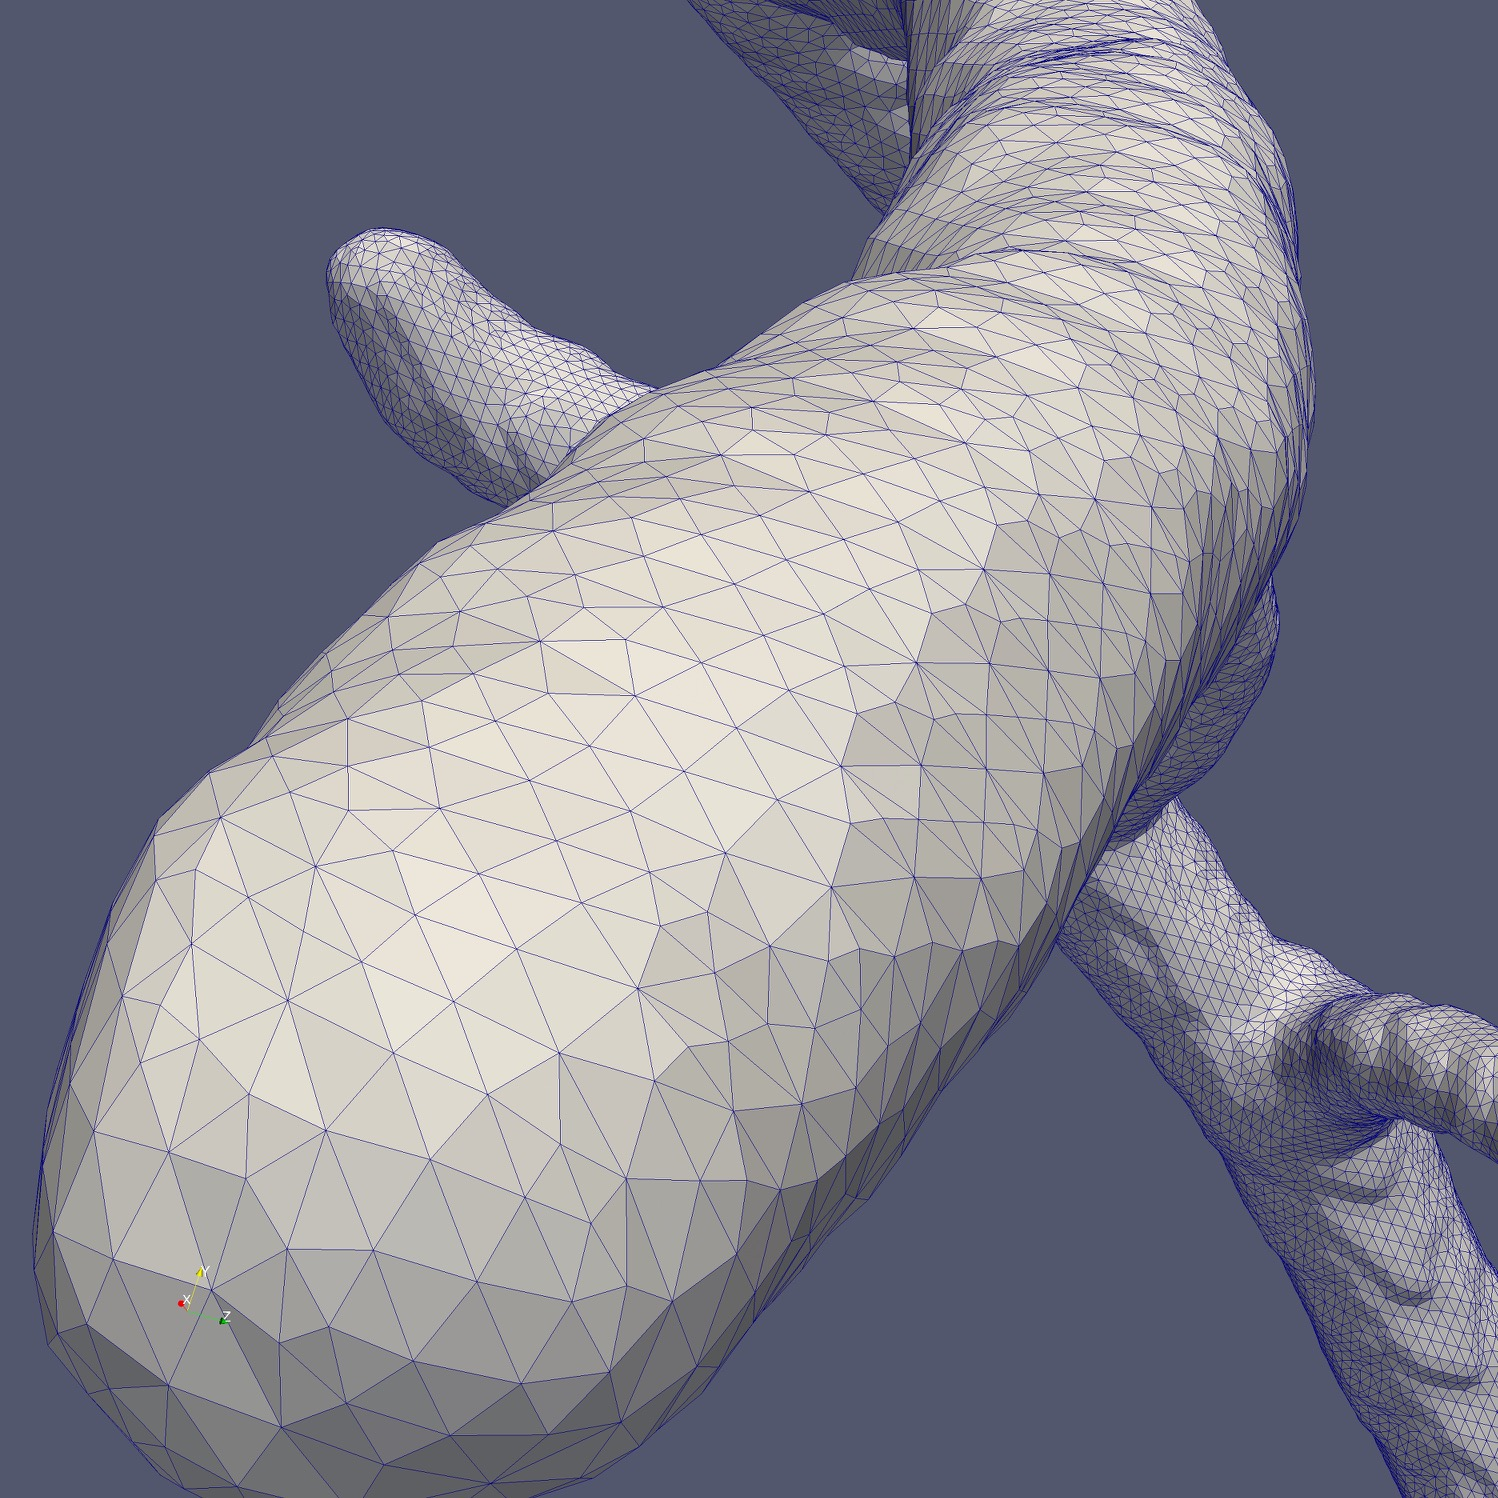
\includegraphics[width=\linewidth,height=\hpart \textheight,keepaspectratio]{\imgpath alt/cu/5_sfi2_wf_cu2}
		\caption*{Surface extraite}
	\end{minipage}
	\begin{minipage}[t]{\figpart \linewidth}
            	\centering
            	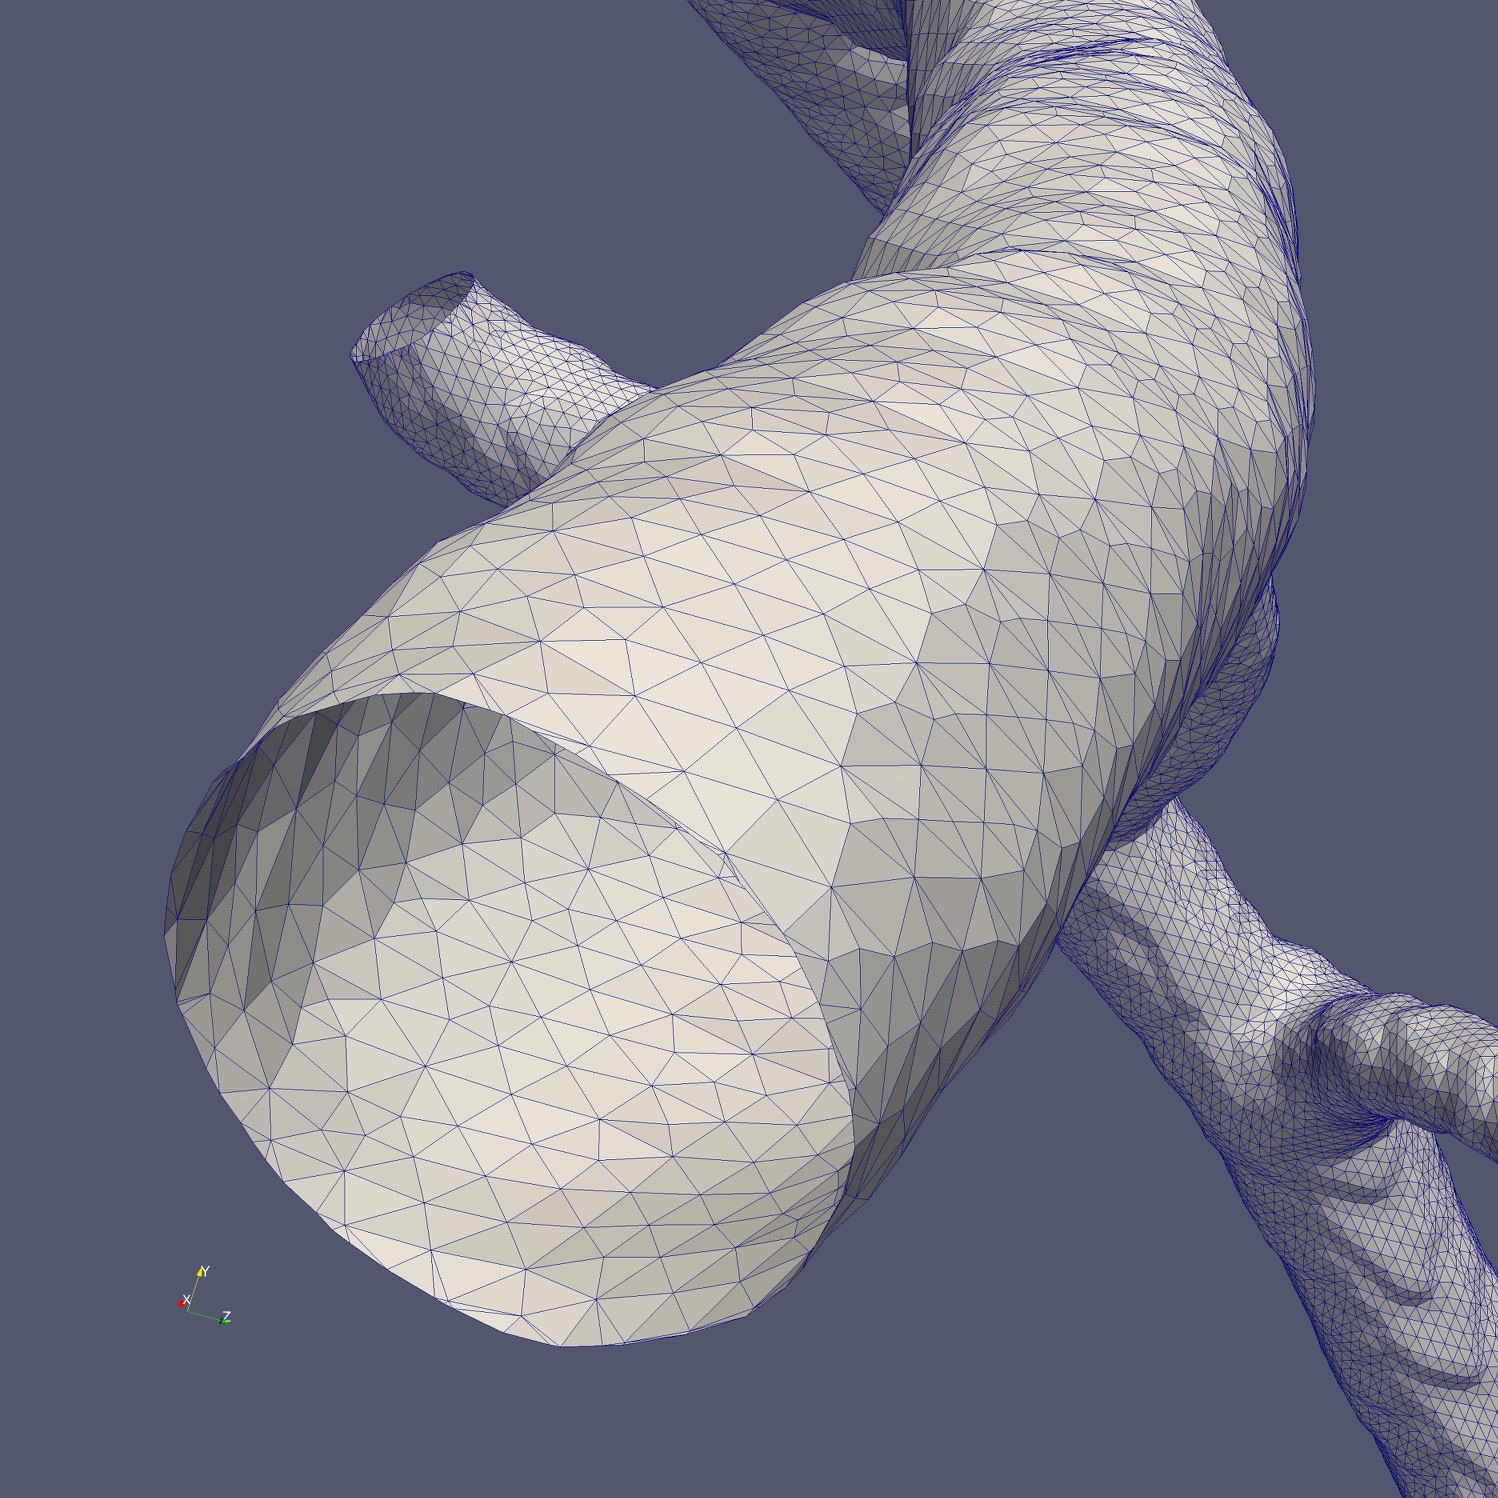
\includegraphics[width=\linewidth,height=\hpart \textheight,keepaspectratio]{\imgpath alt/cu/6_sm_open_wf_cu2}
		\caption*{Ouverture}
	\end{minipage}
	\begin{minipage}[t]{\figpart \linewidth}
            	\centering
            	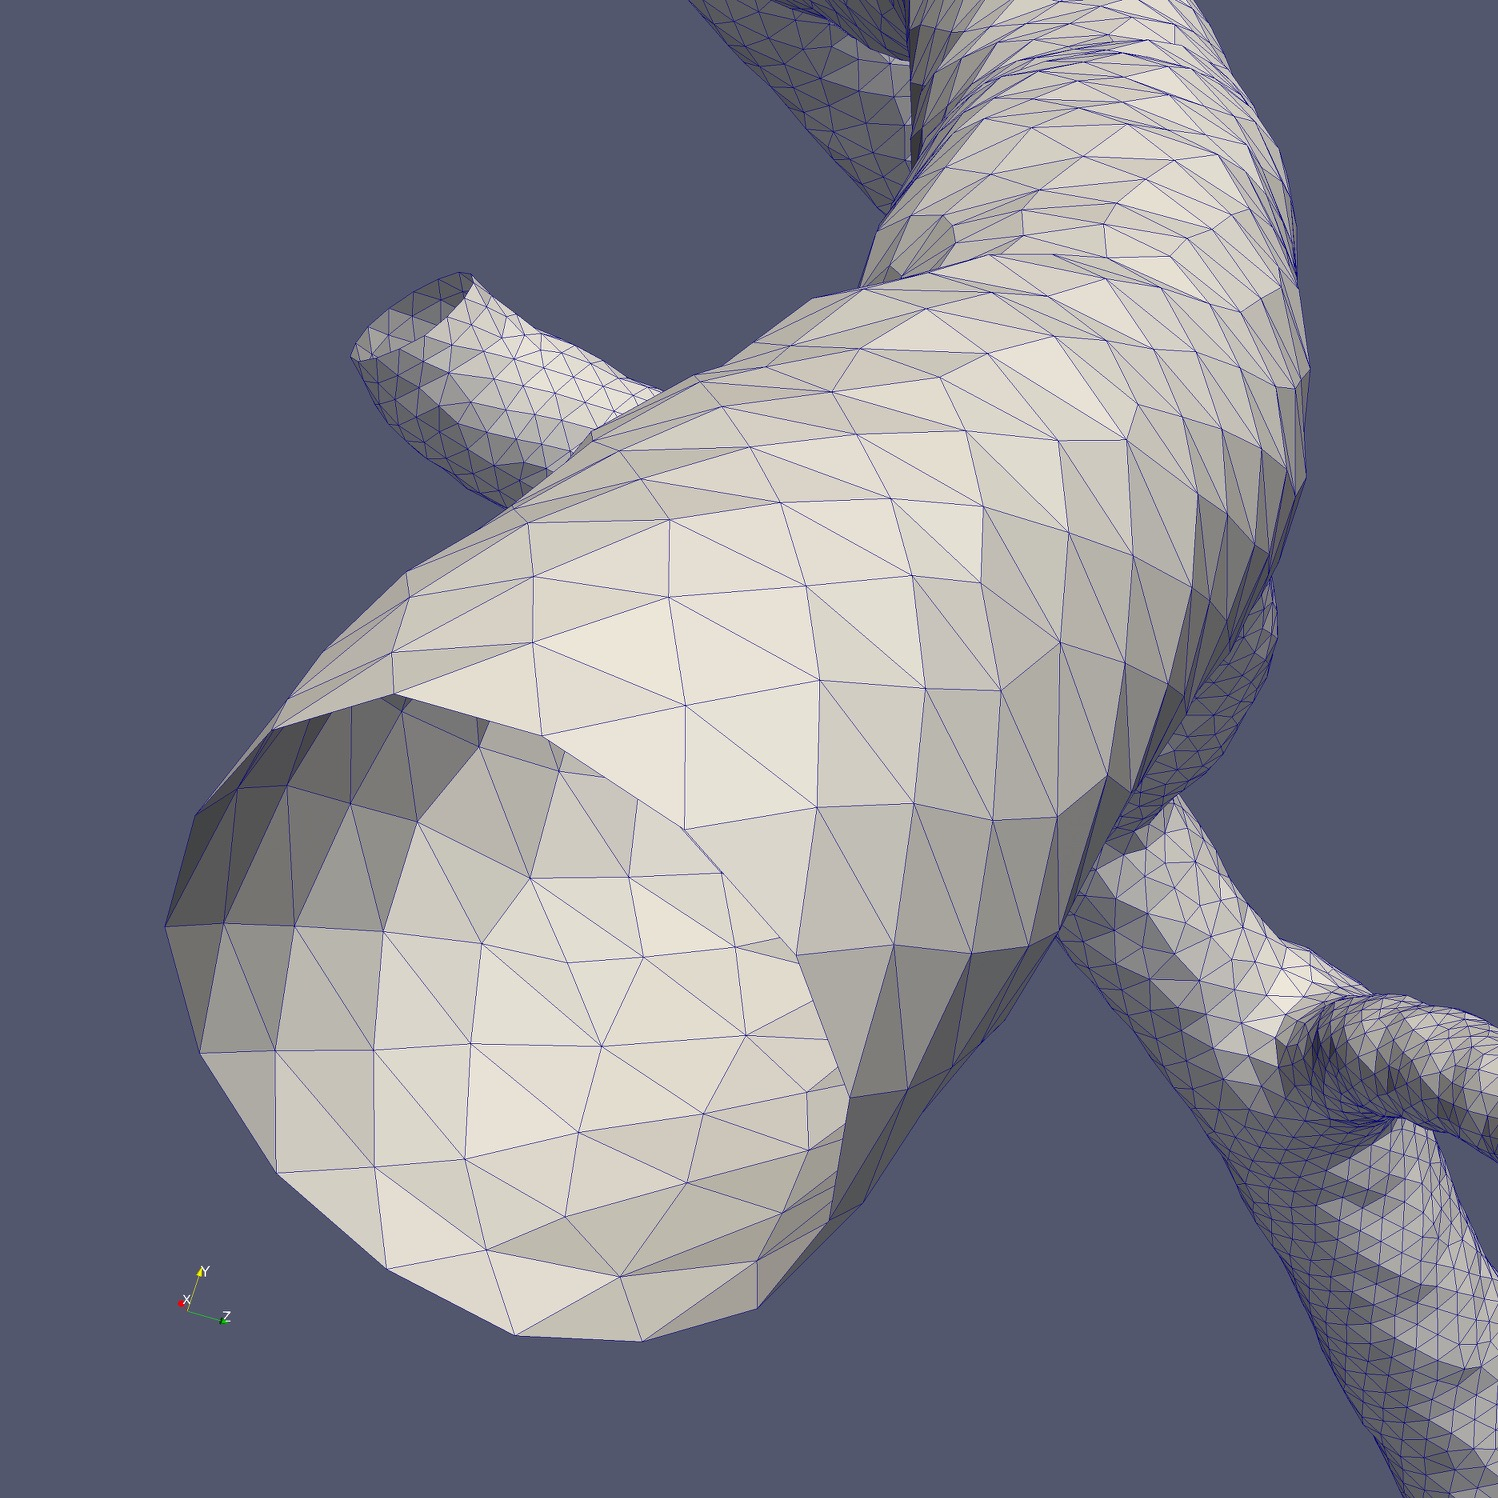
\includegraphics[width=\linewidth,height=\hpart \textheight,keepaspectratio]{\imgpath alt/cu/6_sm_remesh_wf_cu2}
		\caption*{Remaillage surfacique}
	\end{minipage}
	\begin{minipage}[t]{\figpart \linewidth}
            	\centering
            	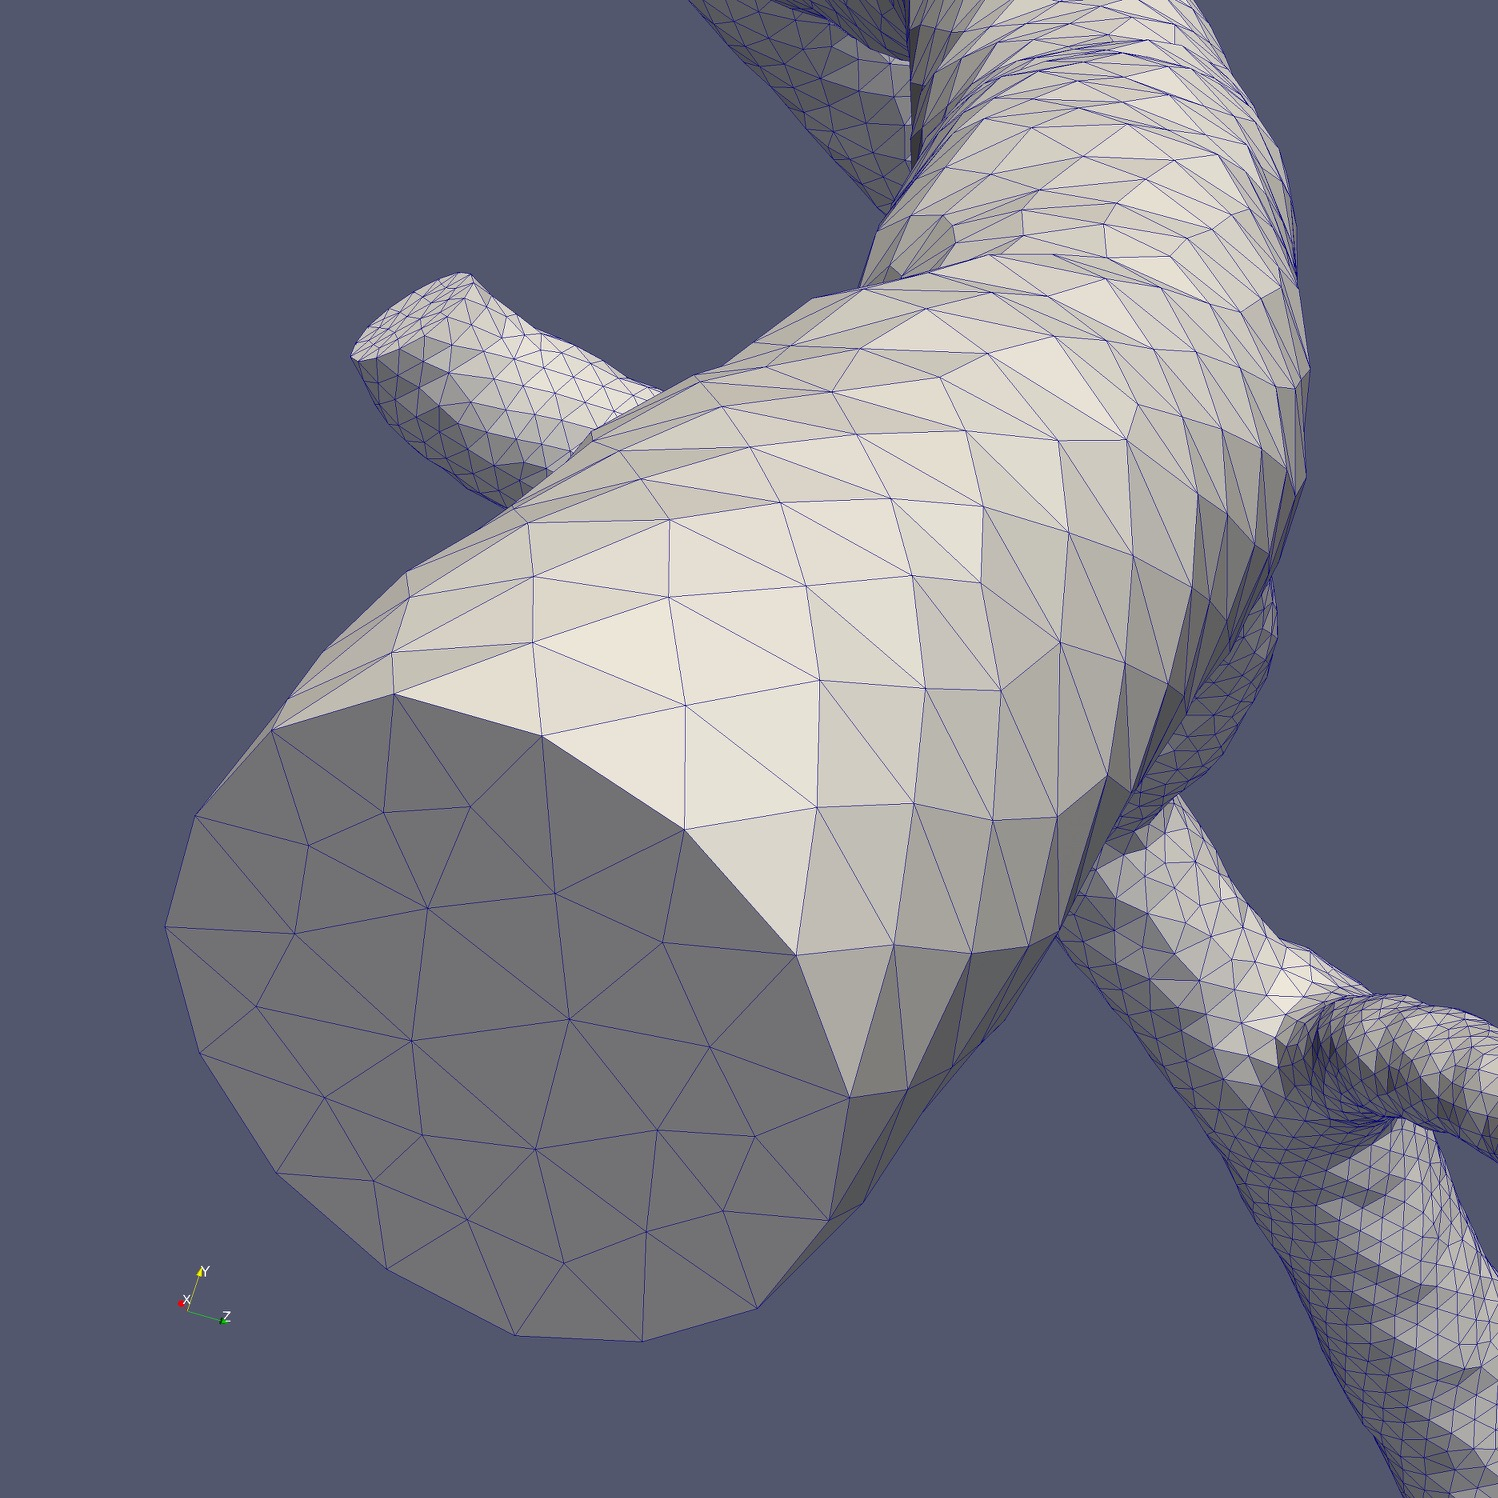
\includegraphics[width=\linewidth,height=\hpart \textheight,keepaspectratio]{\imgpath alt/cu/7_vm_wf_cu2}
		\caption*{Maillage volumique}
	\end{minipage}
	
	\caption{Evolution d'une extrémité de vaisseau sanguin au cours des étapes \ref{arch:sfi2} (\nameref{arch:sfi2}) à \ref{arch:vm} (\nameref{arch:vm}).}
 \end{figure}
\end{center}

\section{Simulation d'écoulements (Feel++)}

Disposant d'un maillage adapté des vaisseaux sanguins, nous pouvons y réaliser des simulations d'écoulements. Ces simulations sont réalisées grâce à Feel++...

\section{Simulation d'angiographies virtuelles (JEMRIS)}

Il est également possible de simuler des IRM de ces modèles reconstruits, afin de réaliser des angiographies virtuelles. Ces simulations sont réalisées grâce à JEMRIS...



%---------------------------------------------------------------------------------------------------------------
%--------------------------------------------------begin def------------------------------------------------
%---------------------------------------------------------------------------------------------------------------

%---------------------------------------------------------------------------------------------------------------
%--------------------------------------------------end def---------------------------------------------------
%---------------------------------------------------------------------------------------------------------------

\renewcommand{\chpath}{3-briques/}
\renewcommand{\imgpath}{\chpath img/}
\renewcommand{\secpath}{\chpath}
\chapter{Briques logicielles}
\label{chap:briques}


\section{Reconstruction de modèle}

\input{\chpath 0-general}

\input{\chpath 1-rorpo}

\input{\chpath 2-sfi}

\input{\chpath 3-mclgui}

\input{\chpath 4-mcl}

\input{\chpath 5-mclm}

\input{\chpath 6-ifcl}

\input{\chpath 7-sfi2}

\input{\chpath 8-sp}

\input{\chpath 9-vp}

\section{Alternatives à l'étude}

\input{\chpath 10-cts}



\renewcommand{\chpath}{4-pipeline/}
\renewcommand{\imgpath}{\chpath img/}
\renewcommand{\secpath}{\chpath}
\chapter{Exécution du pipeline et gestion des résultats}
\label{chap:briques}


\section{Utilisation des scripts}

%\input{\chpath 0-general}

\input{\chpath 1-run}

\input{\chpath 2-master}

%\input{\chpath 3-}



\renewcommand{\chpath}{00-notes/}
\renewcommand{\imgpath}{\chpath img/}
\renewcommand{\secpath}{\chpath}
\chapter{Notes}
\label{chap:notes}

\section{Visualisation de données - \paraview}
Pour visualiser des images \nii dans \paraview, il faut au préalable activer un plugin supportant ce format. 
Le plugin \texttt{AnalyzeNIfTIIO} est intégré à \paraview, mais désactivé par défaut. Pour l'activer, dans l'interface graphique (\paraview 5.0.1), il faut:

\begin{itemize}
\item accéder au menu \texttt{Tools > Manage Plugins...},
\item sélectionner le plugin \texttt{AnalyzeNIfTIIO} dans la liste,
\item cliquer sur \texttt{Load Selected}.
\end{itemize}

En cas de connexion à un serveur \paraview (pvserver), deux listes de plugins seront présentées: une distance (les plugins du serveur) et une locale (ceux de l'instance de \paraview dont l'interface graphique est utilisée). Il suffit d'activer le plugin dans les deux listes.

%\input{\chpath annexe_rorpo}

\nocite{*}
\printbibliography


\end{document}